%%%%% The Validation %%%%%

\chapter{Validation} \label{ch_practice}

The content produced for this thesis has been used in two courses. Evaluation of the feedback provided by students shows that they did like working with the provided environment and that their understanding of the abstractions involved in programming increased somewhat. However, due to limitations in the study setting, further analysis will be required in order to generalize these findings.

Both evaluation rounds were held with classes at Gymnasium Neufeld that we have been teaching ourself. These classes consist of Swiss high school students at ninth and tenth grade (of twelve grades), respectively.


\section{First Round} \label{sc_validation_ca} % 2025-05-12

\subsection{Setting}

The first evaluation round took place in a computer science class consisting of 17 tenth-grade students. This class had, at this point, encountered most of the base curriculum of computer science as required in the Canton of Berne \cite[p.\,145--146]{Erz16}, with only the introduction to systems architecture missing.

Specifically, the introduction to programming had been taught using Processing with Python syntax inside the Processing \ac{IDE}, so students already had the desired prior experience in programming with Processing. Additionally, the class had written their last partial exam five weeks prior, which had, among other topics, contained a repetition sequence on binary numbers and encodings.

Contrary to the suggestions in \ref{sc_lesson_ca}, the introduction to computer architecture was being taught bottom up, loosely following Nisan and Schocken's ideas \cite{Nis21} in a significantly abbreviated course of only 6 instead of 12 weeks.\footnote{The reason for this was originally the same as Nisan and Schocken's, \ie building concepts on a solid foundation.}

At the point where the environment developed for this thesis was introduced, students already had encountered some of the foundational building blocks of a modern microchip: transistors built out of semiconductors, logic gates, and circuits up to an adder circuit as the basis of an \ac{ALU}.

The plan was thus to connect the already encountered foundation with their knowledge about programming by revealing and discussing several of the involved abstraction layers. Due to time constraints, only an excerpt of the sequence proposed in \ref{sc_lesson_ca} could be realized.

On the day of the lessons, 14 of the 17 students were present. At the start of the first lesson, \ac{GT} was distributed through the school's OneDrive infrastructure. The \ac{GT} environment was then introduced similar to \ref{ssc_lesson_gt}, but, as was the rest of the lessons, mostly in a self-guided way, with instructions being provided in \ac{GT} notebook pages.\footnote{The exact state of the materials is available at \url{https://github.com/zeniko/processing-abstractions/tree/thesis} in commit \ct{71047704f7f70c13d3d01ac520618e15d569274f} of May 12th.}

During the lessons, students were supported where needed but left to work at their own individual pace, which the reduced number of students allowed for. Afterwards, a questionnaire was distributed to students to receive their own feedback in addition to the collected observations.\footnote{See appendix \ref{app_questionnaire_1} on page \pageref{app_questionnaire_1} for the full questionnaire.}

At least one of the students missing the lessons was successfully able to work on the provided content on her own.


\subsection{Observations}

During the time available, students have been able to work on their own for large amounts of time with only a few common issues occurring. The interactive notebook pages seemed to allow for creating an effective teaching environment.

Additionally, many students have been observed to actively tinker with the interactive elements, as was desired and was to be expected from providing an environment for live programming and exploration. Except for a few hiccups where the \ac{GT} notebook pages stopped updating (for which the usual cure of reloading helped), the interactivity worked reliably -- up to the point where students found it so engaging that they got sidetracked by writing and modifying programs for their effect instead of the changes to the views for different layers.

Nonetheless, the more active students have been able to work through the subject matter on their own, whereas less interested students had to be motivated from time to time to continue reading and interacting. With students being able to work on their own, we had ample time for supporting these students with instructions, hints, and some motivating background information.

Despite their prior Processing knowledge, students were sometimes out of their depth when changes to a Processing program were asked for. In a next round, this sequence would have to be placed closer to a programming sequence with Processing, or at least a brief repetition of just using Processing would be helpful.

What caused most issues was the way \ac{GT} opened notebook pages from content links in a new page adjacent to the previous one, hiding the table of contents in the process, instead of opening them in place of the previous page, as students were used to from web browsers. This caused students to lose track of the pages they were supposed to be working on, to the point of occasionally skipping part of the assigned content. This happened despite the brief introduction to working with \ac{GT} where closing additional pages and getting the table of contents back was an explicit introductory task.

The overall impression of the lessons was that students had been working productively, mostly autonomously, and at their own pace with the teaching materials provided.


\subsection{Student Feedback}

In order to verify our own observations, students were provided with a questionnaire. Of the 17 students, however, only 11 returned feedback despite frequent reminders. Therefore, the following yields, at best, qualitative results.\footnote{Questionnaire data in anonymized form is available at \url{https://github.com/zeniko/gyminf-thesis/blob/main/data/data_6_1.csv}.}

Additionally, three weeks later, the students have written another partial exam with individual tasks referring to the lessons with \ac{GT}.

Student feedback shows the following: Students quite liked working with the provided environment (grading it mostly 4/5 with a bootstrapped 95\%-confidence interval of between 3 and 4) and reported that it worked reasonably well but not yet perfectly (most students grading it either 3/5 or 4/5 with a bootstrapped 95\%-confidence interval of between 2 and 4). This is consistent with our own observations.

\begin{cfigure}[fig_plots_27ga]{Answers to questionnaire questions 1 and 3: How well did you like working with this environment? How well do you think you could explain what you have learned today?}
\begin{tikzpicture}[baseline=(current axis.center), scale=0.85]
\begin{axis}[
	y=1cm,
	ytick={1,2},
	yticklabels={Q1,Q3},
	xtick={1,2,3,4,5},
	xmin=1,
	xmax=5,
	xlabel={1 = not at all, 5 = very much},
]
	\addplot+[boxplot] table [row sep=\\,y index=0] {
		Q1 \\ 4 \\ 4 \\ 3 \\ 3 \\ 4 \\ 4 \\ 4 \\ 4 \\ 3 \\
	};
	\addplot+[boxplot] table [row sep=\\,y index=0] {
		Q3 \\ 4 \\ 3 \\ 2 \\ 1 \\ 2 \\ 3 \\ 2 \\ 3 \\ 2 \\
	};
\end{axis}
\end{tikzpicture}
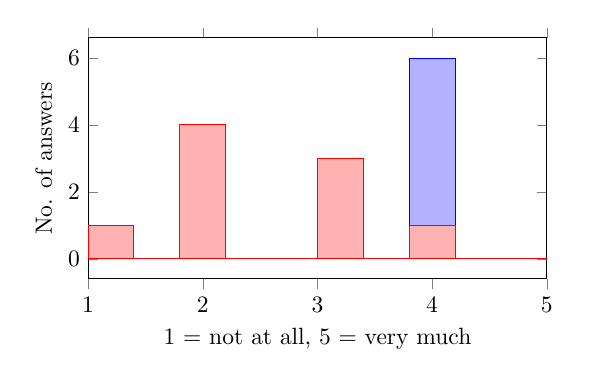
\begin{tikzpicture}[baseline=(current axis.center), scale=0.85]
\begin{axis}[
	ybar,
	y=0.5cm,
	xmin=1,
	xmax=5,
	xlabel={1 = not at all, 5 = very much},
	ylabel={No. of answers}
]
	\addplot+[hist] table [row sep=\\,y index=0] {
		Q1 \\ 4 \\ 4 \\ 3 \\ 3 \\ 4 \\ 4 \\ 4 \\ 4 \\ 3 \\
	};
	\addplot+[hist] table [row sep=\\,y index=0] {
		Q3 \\ 4 \\ 3 \\ 2 \\ 1 \\ 2 \\ 3 \\ 2 \\ 3 \\ 2 \\
	};
\end{axis}
\end{tikzpicture}

\end{cfigure}

Part of the reason for their liking working this way might be due to them considering programming one of the best parts of computer science. This shows in the question about what students considered to be their ``highlight'' of the computer science course, to which half the students responded with either programming in general or the game programming project in particular.

When asked explicitly about the usefulness of the various abstraction views provided, students noted that they were very useful (mostly grading it either 4/5 or 5/5 with a bootstrapped 95\%-confidence interval of between 4 and 5). Also, a majority of students indicated repeatedly interacting actively with the program samples.

What they liked the most was being able to work at their own speed (and optionally being able to decide for themselves whether to work together or alone). This is due to guidance from the environment, which allows teachers to introduce tasks for students to explore autonomously in order to build understanding. One student even explicitly noted that being able to see changes reflected instantly was gratifying.

Their main concern was two of the more engaged students, noting that some explanations were not yet as clear as they could be, requiring them to ask instead of being able to work for themselves. Additionally, the quickest working student would have preferred fewer links within notebook pages, reducing the annoyance of losing the table of contents from web browser habits.

Students gave their feedback between one day and one week after the lesson. When asked to reword the learned content in their own words, most of them failed to describe entirely correctly what they had learned. Had their answers been graded, all but one student would have only been awarded at most half the points. Also, the desired connection with the previously taught content about transistors and logic gates remained unclear, with this time all students getting at most half the points.

Finally, the partial exam resulted in students answering questions related to these lessons correctly to only about 46\%. The result does, however, weakly correlate with students' general commitment (measured by their final grade, yielding a rank correlation of $0.48$).


\subsection{Learnings}

The desired effect of having students better understand abstraction layers seems not to have yet been achieved. While the environment was engaging and led students to explore on their own, explanations will have to be expanded and made clearer for students to be able to fully understand what they are shown.

Part of the issue is, however, that time was too short and the implementation was not fully fledged, so these findings might also be due to both of these. So further analysis will be required, and the environment will have to be tested at a larger scale with the other classes with better integration in the curriculum (as suggested by the author in \ref{sc_lesson_ca}).

At least some of the technical issues observed have since been remedied, although mostly by more explicitly telling students what to do when issues arise.

Also, since \ac{GT} runs purely on the students' own computers, their progress can't be observed other than by monitoring their screens. For this, either a separate progress tracker (such as \url{https://learningview.org/}) would have to be used or a sequence of short tests, not only checking for progress of reading but also of comprehension.



\section{Second Round} \label{sc_validation_compiler} % 2025-06-30

\subsection{Setting}

The second evaluation round took place in a computer science class consisting of 23 ninth-grade students. At that point, this class had passed about half the required content of the base curriculum to computer science \cite[p.\,145--146]{Erz16}, including application usage, various encodings, algorithms, and an introduction to programming using Processing eight weeks prior.\footnote{For unfortunate timing reasons, the programming project had to be postponed.}

Two lessons at the end of the school year could be set aside for an introduction to compilers as part of this thesis. These would usually have to be placed later in the curriculum, either together with the introduction to computer architecture or beyond.

The plan was to implement an excerpt of the course from \ref{sc_lesson_compiler}. As a quick overview, Human Resource Machine was used for introducing students to the limitations of machine language and motivating the need for compiling programs before executing them on actual hardware. Afterwards, \ac{GT} was introduced with additional stress on using the table of contents for navigation. Finally, students were asked to work through the provided content at their own speed.\footnote{The exact state of the materials is available at \url{https://github.com/zeniko/processing-abstractions/tree/thesis} in commit \ct{6e22cddb176fdd46d410b9db40496bafa8a59c08} of June 30th.} Towards the end of the lessons, students were given time to fill out a questionnaire.\footnote{See appendix \ref{app_questionnaire_2} on page \pageref{app_questionnaire_2} for the full questionnaire.}

One unplanned limitation of these lessons was summer being early with high temperatures. As a consequence, only 15 of the 23 students were present for the introduction, and the introduction had to be moved to a different, cooler location.


\subsection{Observations}

In general, the students worked reliably with the content provided. In particular, this group seemed to quite naturally take notes within the \ac{GT} notebook pages, making the content their own.

Working speed again was heterogeneous, but some smaller groups formed, which supported each other. One student in particular volunteered repeatedly to help his peers.

Despite programming with Processing being rather fresh, fewer students seemed to interact with the sample programs provided, despite tasks asking them to do so explicitly. About half the students seemed content to observe views as static content.

This group had more problems getting \ac{GT} even to run. Even though these students already had successfully downloaded and used apps on their own, and despite a separate \ac{GT} launcher in the top-level folder being provided, many failed to start \ac{GT} on their own.

Part of these issues might, however, relate to high temperatures, making it more difficult for students to focus.


\subsection{Student Feedback}

Of the 15 students present, 14 managed to hand in the questionnaire (with the last student's computer previously running out of battery power).\footnote{Questionnaire data in anonymized form is available at \url{https://github.com/zeniko/gyminf-thesis/blob/main/data/data_6_2.csv}.} With this small number of answers, again, no reasonable quantitative evaluation is possible.

The students' answers show that many of them (12/15) have worked more slowly than expected, only learning about lexer and parser in the hour provided. Also, disappointingly, only two of the 15 were at least somewhat confident that they would be able to explain the learned content to their peers.

\begin{cfigure}[fig_plots_28ga]{Answers to questionnaire questions 1 and 3: How well did you like working with this environment? How well do you think you could explain what you have learned today?}
\begin{tikzpicture}[baseline=(current axis.center), scale=0.9]
\begin{axis}[
	y=1cm,
	ytick={1,2},
	yticklabels={Q1,Q3},
	xtick={1,2,3,4,5},
	xmax=5,
]
	\addplot+[boxplot] table [row sep=\\,y index=0] {
		Q1 \\ 4 \\ 3 \\ 1 \\ 4 \\ 3 \\ 2 \\ 3 \\ 3 \\ 4 \\ 2 \\ 2 \\ 3 \\ 3 \\ 2 \\
	};
	\addplot+[boxplot] table [row sep=\\,y index=0] {
		Q3 \\ 2 \\ 1 \\ 1 \\ 3 \\ 1 \\ 2 \\ 2 \\ 2 \\ 4 \\ 2 \\ 2 \\ 2 \\ 1 \\ 1 \\
	};
\end{axis}
\end{tikzpicture}
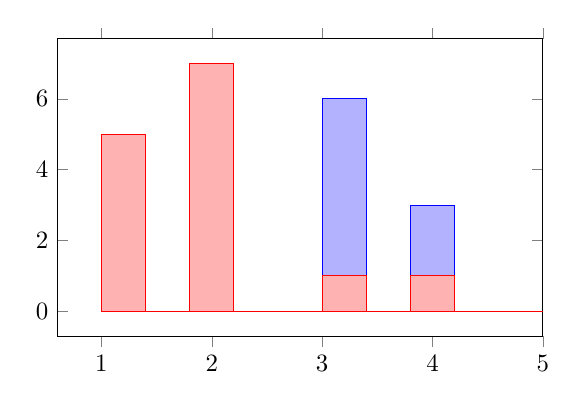
\begin{tikzpicture}[baseline=(current axis.center), scale=0.9]
\begin{axis}[
	ybar,
	y=0.5cm,
	xmax=5,
]
	\addplot+[hist] table [row sep=\\,y index=0] {
		Q1 \\ 4 \\ 3 \\ 1 \\ 4 \\ 3 \\ 2 \\ 3 \\ 3 \\ 4 \\ 2 \\ 2 \\ 3 \\ 3 \\ 2 \\
	};
	\addplot+[hist] table [row sep=\\,y index=0] {
		Q3 \\ 2 \\ 1 \\ 1 \\ 3 \\ 1 \\ 2 \\ 2 \\ 2 \\ 4 \\ 2 \\ 2 \\ 2 \\ 1 \\ 1 \\
	};
\end{axis}
\end{tikzpicture}

\end{cfigure}

This is consistent with students failing to answer basic questions about the need for compilation (half of them not answering or answering entirely wrong), but slightly better about the roles of lexer and parser (one third answering correctly and one third getting at least half of their answer correct).

It is difficult to judge how much of this is due to the environment not meeting expectations and how much is due to summer, as when asked explicitly about their thoughts on the provided environment, students wrongly referred to the general learning setting instead of the Processing Abstractions environment.

The only general remark that students agreed on was that they had enjoyed programming (11/15), which, in contrast to the other class (see \ref{sc_validation_ca}), however, still did not result in as much tinkering (with only 4/15 students reportedly playing around and exploring).


\subsection{Learnings}

Unfortunately, not much was to be learned from this test, mostly due to environmental factors. A repetition of this setting will thus be required at a later time. At least the content that students actually got to seems to have been sufficiently clear for them to somewhat understand.
